\chapter{Integração Redmine e Activiti BPM}\label{chp:integracao_redmine_activiti}


\section{Cenário da Integração}\label{sec:cenario-integracao}

A utilização do Redmine como gerenciador de processos acaba sendo limitada, como foi descrito no capítulo \ref{chp:redmine}, já que não possui efetivamente um motor de processos BPM. Ainda assim, a possibilidade de extensão e desenvolvimento de novas funcionalidades no Redmine sugere que o mesmo possa ser evoluído para o atendimento de processos mais complexos, ao mesmo tempo em que suas vantagens de portal e atendimento de processos mais simples são mantidos.

Com o objetivo de evoluir o Redmine para o atendimento de fluxos de trabalho mais complexos, torna-se necessário o desenvolvimento de um motor de processos mais robusto e que possibilite novas opções e configurações de fluxos de trabalho na ferramenta. Entretanto, uma solução deste porte acaba por convergir em problemas solucionados por ferramentas BPMS, que permitem a modelagem e execução de processos complexos.

A utilização de BPMS a para automatização de processos de negócio traz diversas vantagens, conforme apresentado na seção \ref{sec:automatizacao-processos-bpms}. Além das vantagens já citadas, ao utilizar a notação BPMN, o motor de processos reduz a necessidade do desenvolvimento de funcionalidades específicas que acabam sendo possíveis simplesmente pela modelagem na notação. A implementação de fluxos de trabalho mais complexos acabaria sendo possível no Redmine somente com o desenvolvimento de plugins ou mudanças no código-fonte principal; o que seria custoso, arriscado e imanutenível a longo prazo.

Boa parte das aplicações BPMS mais robustas oferecem algum tipo de portal, onde ocorrem basicamente as interações com as tarefas humanas, e também APIs para manipulação dos processos, o que permite a integração com diferentes interfaces e aplicações. Entretanto, nem sempre esses portais possuem uma interface tão amigável para o usuário, ou são adaptados a dispositivos móveis como \textit{smartphones} ou \textit{tablets}, ou são de fácil customização. Essas são características positivas encontradas no Redmine, que conta com mais de 50 temas prontos para uso na lista oficial\cite{redmine_themes}, além de possuir uma estrutura bem organizada para customização e criação de novos \textit{layouts}. 

O Redmine também possui um excelente suporte à geração automática de formulários pela associação de campos customizados tipados às tarefas, como por exemplo datas, caixas de seleção e texto. Comparativamente, a implantação de processos mais simples pelo Redmine acaba sendo mais rápida e mais fácil de ser mantida do que em ferramentas BPMS, já que não é necessário nenhuma modelagem em notação específica, \textit{deploy} de processos ou desenvolvimento de formulários; tudo é feito facilmente pela interface web. 

Neste sentido, torna-se interessante propor uma solução que aproveite todas as vantagens de portal e implantação de processos de negócio mais simples do Redmine, mas que também ofereça todo o poder e flexibilidade de modelagem de processos mais complexos oferecidos por ferramentas BPMS. Nasce assim a ideia de propor uma solução integrada para a automatização de processos de negócio, através da integração do Redmine com uma ferramenta BPMS.

\section{Integração Genérica}\label{sec:cenario-integracao-genérica}

 
 Pensando na possibilidade de utilizar qualquer plataforma BPMS integrada ao Redmine, decidimos avaliar a utilização de ferramentas ESB\cite{esb} de forma a facilitar a construção de uma interface única de comunicação com o Redmine. Conforme definido em publicação do O'Reilly\cite{oreilly_esb}, ESB é uma plataforma de integração baseada em padrões que combina mensagens, serviços web, transformação de dados e roteamento inteligente para conectar de forma confiável e coordenar a interação de um número significativo de aplicações e serviços. Assim, bastaria o trabalho de integrar o BPMS escolhido com este barramento, e assim o Redmine estaria capacitado a orquestrar fluxos de trabalho mais complexos utilizando qualquer BPMS de mercado. A figura \ref{fig:arquitetura_integracao_generica_redmine_bpm}  apresenta o modelo de arquitetura proposto para a integração genérica do Redmine com BPMS.

\begin{figure}[H]
\centering
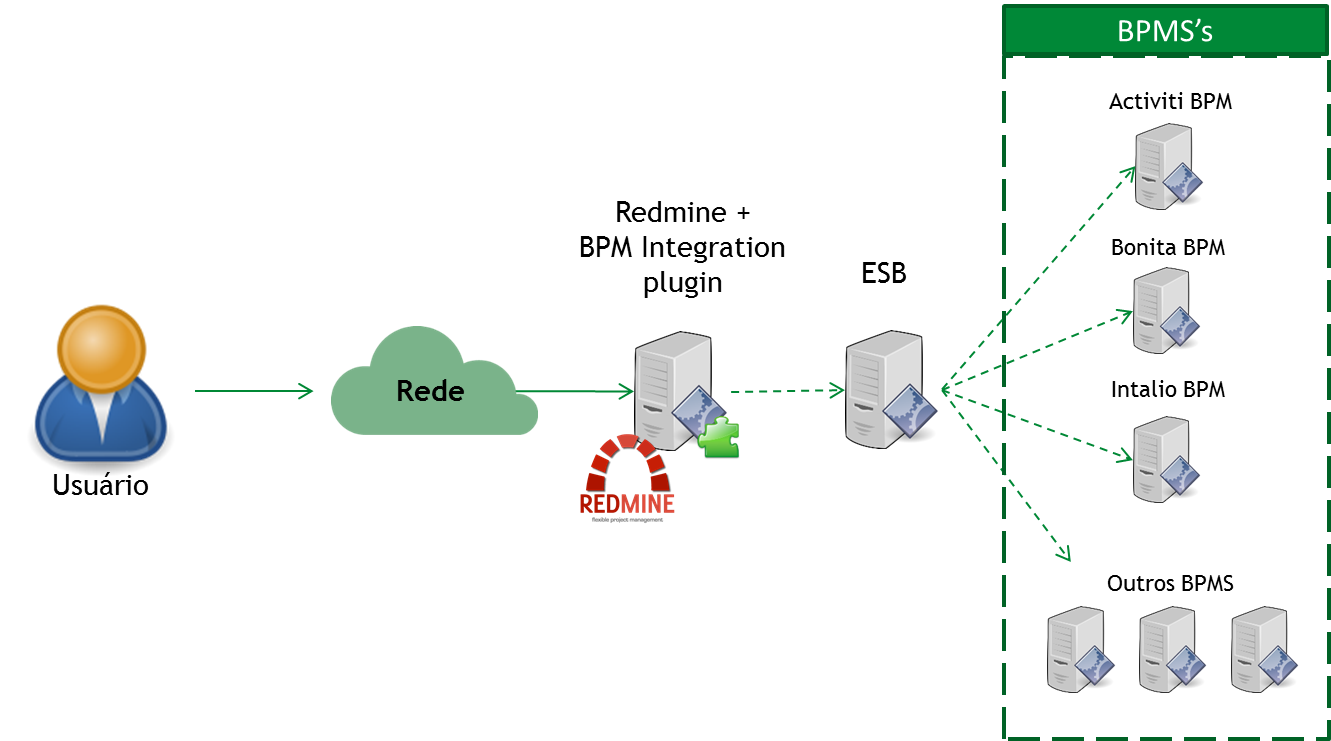
\includegraphics[width=1\textwidth]{imagens/arquitetura_proposta_inicialmente_bpm_integration.png}
\caption{Arquitetura proposta de integração genérica entre Redmine e BPMS's}
\label{fig:arquitetura_integracao_generica_redmine_bpm}
\end{figure}

Iniciamos o desenvolvimento deste barramento através da escolha de um ESB e pelo menos dois BPMS para validar a construção desta interface. Para o ESB, optamos pelo Mule ESB\cite{mule} que possui uma versão gratuita e está posicionado como uma das melhores ferramentas do seguimento de integração empresarial, segundo o quadrante mágico anual da Gartner\cite{mule_gartner}. Para o BPMS, optamos por duas ferramentas com versões gratuitas, desenvolvidas na linguaguem Java e com uma boa interface REST: Activiti BPM\cite{bpm_activiti} e Bonita BPM\cite{bpm_bonita}.

O primeiro serviço escolhido para modelagem no barramento foi o responsável por disparar um novo processo no BPMS. Consistiria basicamente na disponibilização de um serviço REST, com parâmetros comuns às APIs de ambos os BPMS para que um novo processo fosse iniciado na plataforma escolhida. Apesar de um esforço considerável para a construção deste primeiro serviço, foi desenvolvido com sucesso.  

Entretanto, este piloto foi suficiente para identificarmos logo no início que haveria um grande esforço para a construção deste barramento, uma vez que exigiria uma alta complexidade na modelagem pelas diferenças entre as APIs e a necessidade de conhecimento a fundo de diferentes serviços para que a solução fosse realmente genérica. Percebemos fundamentalmente que esta solução exigiria um altíssimo esforço de desenvolvimento e modelagem, e que nos afastaríamos do objetivo central deste trabalho, que é prover um motor de processos mais complexo para o Redmine. 

Nesse sentido, decidimos abortar a construção desta interface genérica, e partirmos para uma solução de menor complexidade, mas que provesse o ganho almejado com a solução integrada do BPMS ao Redmine.

\section{Integração Activiti BPM}\label{sec:cenario-integracao-activiti}

Dada a complexidade de criação dessa interface genérica, decidimos desenvolver a integração do Redmine com um BPMS específico de mercado. Nesse cenário, diversas dificuldades envolvidas ao processo de generalização deixaram de ser preocupação, e permitiram que o desenvolvimento fosse mais focado na solução do problema inicial, que é trazer mais flexibilidade e alternativas de fluxo de trabalho para o Redmine.

Sendo assim, foi necessário definir um BPMS de mercado que atendesse a alguns critérios. O motor deveria ser gratuito e de código aberto, estando assim alinhado com a proposta open-source do Redmine. Além disso, seria fundamental que a ferramenta fosse leve, extensível e com uma API de fácil utilização e boa documentação, possibilitando assim um rápido entendimento da plataforma e abertura para qualquer modificação ou extensão necessária na ferramenta. Seria desejável também que a ferramenta estivesse em constante evolução e fosse suportada por uma comunidade ativa e que pudesse oferecer suporte para dúvidas encontradas durante o processo de integração.

Ao avaliarmos as possibilidades, identificamos uma ferramenta que se encaixava bastante nos critérios adotados, o Activiti BPM. O Activiti BPM é uma ferramenta de código aberto, compartilhado no GitHub\cite{activiti_github}, possui extensa documentação\cite{activiti-userguide} e dispobiliza uma API REST (arquitetura oficialmente adotada pelo \textit{framework} Ruby on Rails desde sua versão 2.0, lançada em dezembro de 2007\cite{rails_rest_support}) facilitando a comunicação com o Redmine, que é escrito nesta linguagem. 

\section{Customização do Redmine}\label{sec:integracao_redmine_activiti-implementacao}

Para atingir este objetivo, criamos um plugin para o Redmine que possibilita a comunicação com o Activiti BPM. Nas próximas sessões, descreveremos o processo de construção deste plugin e como utilizá-lo. Neste trabalho utilizamos a versão 3.1 do Redmine\cite{redmine31}.

\subsection{Arquitetura da solução}\label{sec:integracao_redmine_activiti_implementacao-arquitetura}

A integração tem por objetivo centralizar o máximo de funcionalidades no Redmine, deixando transparente tanto para o usuário comum como o gestor, a existência de um motor BPM por trás.

\begin{figure}[H]
\centering
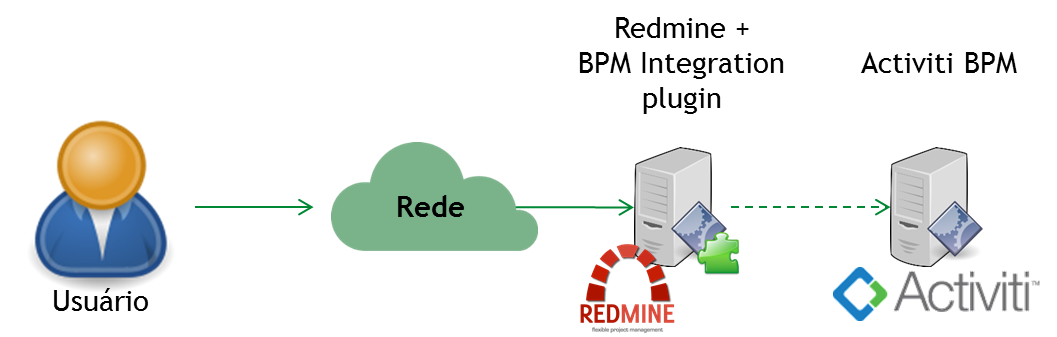
\includegraphics[width=1\textwidth]{imagens/arquitetura_desenvolvida_bpm_integration.png}
\caption{Arquitetura da integração entre Redmine e Activiti}
\label{fig:arquitetura_integracao_redmine_bpm}
\end{figure}

A figura \ref{fig:arquitetura_integracao_redmine_bpm} ilustra a arquitetura da solução de integração proposta. O usuário continua a interagir diretamente com o Redmine da mesma maneira que fazia antes da criação do \textit{plugin}. O Redmine, então, se comunica com o Actitivi pela sua API disponibilizada através de um Web Service REST.

A abordagem utilizada visou concentrar todo o esforço de integração do lado do Redmine, sem a necessidade de customização do Activiti BPM, tornando transparente para ele, também, que o Redmine está sendo usado como sua interface com os usuários finais.
    

\subsection{Linguagens}\label{sec:integracao_redmine_activiti_implementacao_detalhes_desenvolvimento_linguagens}

O plugin desenvolvido para Redmine foi desenvolvido em Ruby\cite{ruby-lang}, utilizando a framework Rails\cite{rails}.
As modificações feitas no Activiti BPM foram feitas em Java, a linguagem que em que este foi desenvolvido.

\subsection{Banco de dados}\label{sec:integracao_redmine_activiti_implementacao__bd}

O banco de dados utilizado neste trabalho foi o MySQL 5.7. Este é o banco mais utilizado e testado com o Redmine pela comunidade.

\subsection{Comunicação entre o Redmine e Activiti}\label{sec:integracao_redmine_activiti_implementacao_sincronizacao}

Para possibilitar a comunicação entre o Activiti BPM e o Redmine foi desenvolvido um mecanismo de sincronização.
Toda a comunicação foi desenhada de forma que o Redmine funcionasse como uma interface do Activiti BPM. Portanto, o primeiro sempre consome a API REST do BPMS para disparar ações, ou ler informações do mesmo.

\subsubsection{Definição de processo}

Para o Redmine assumir a função de interface principal do Activiti BPM, foi desenvolvida a funcionalidade do Activiti Explorer que permite ao usuário fazer o deploy de um processo através dele, uma ação que faz upload da modelagem BPMN e disponibiliza o processo para ser iniciado. Esta funcionalidade dispara um serviço que acessa a API REST do Activiti BPM, executando uma requisição POST que efetivamente executa o deploy, adicionando a modelagem do processo em questão à lista de definições de processos ativos, que podem ser iniciados.

Após executado o serviço, é iniciado um job que busca a definição à partir do deployment\_id. As informações do processo que são recuperadas consistem das tarefas humanas definidas, campos de formulário, variáveis de processo e outros detalhes.
Na figura \ref{fig:process_list} é possível ver a tela da lista de processos ativos desenvolvida no plugin BPM Integration.

\begin{figure}[H]
\centering
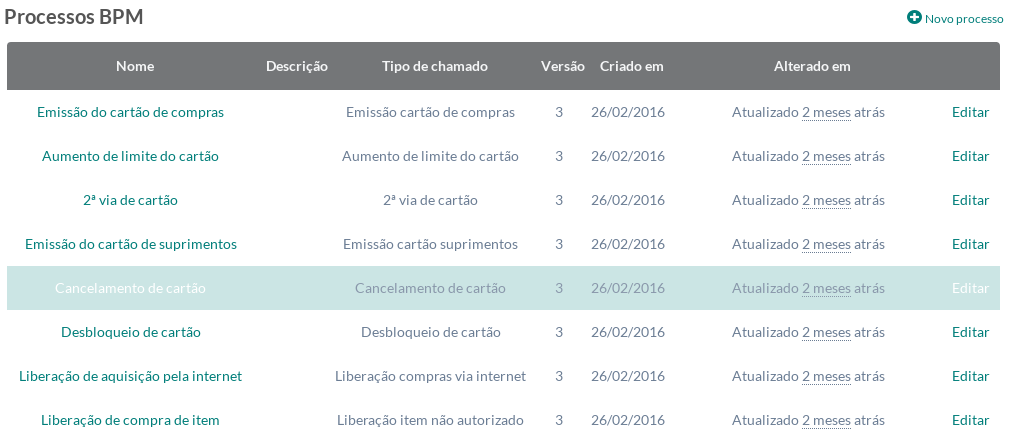
\includegraphics[width=1\textwidth]{imagens/plugin_process_list.png}
\caption{Lista de processos ativos na tela do plugin do Redmine}
\label{fig:process_list}
\end{figure}

\subsubsection{Inicialização de um processo}\label{sec:integracao_redmine_activiti_sincronizacao_inicializacao_processo}
Sempre que uma tarefa é criada, caso ela esteja vinculada a um processo BPM (configuração provida pelo plugin), um serviço é disparado. Este serviço executa uma requisição POST à API REST do Activiti, que dispara uma nova instancia de um processo no mesmo. A requisição carrega as informações da tarefa a ser criada, inclusive os valores dos campos customizados, que foram mapeados para algum campo de formulário da definição de processo do BPMS.

A figura abaixo mostra a tela de criação de tarefas no Redmine, que dispara um novo processo.

\begin{figure}[H]
\centering
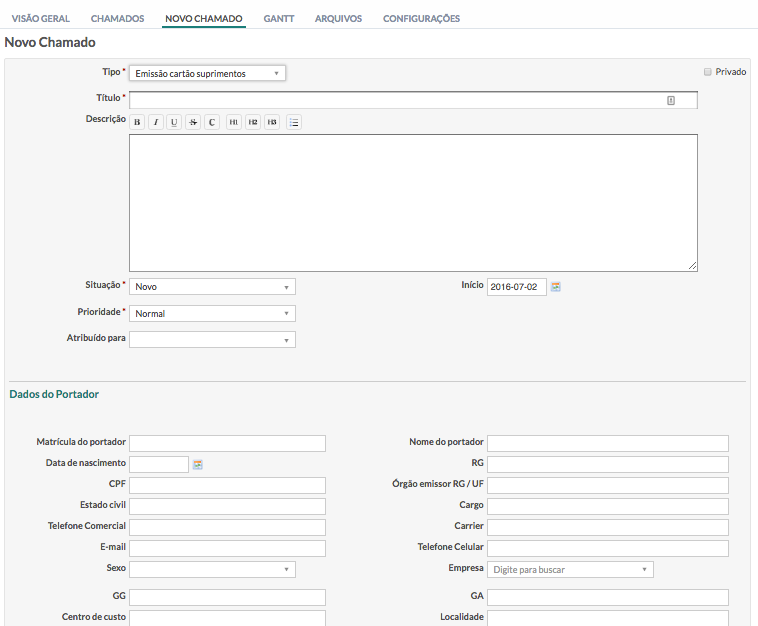
\includegraphics[width=1\textwidth]{imagens/redmine_new_issue.png}
\caption{Tela de criação de tarefas no Redmine}
\label{fig:new_issue}
\end{figure}

Os valores preenchidos para os campos padrão do Redmine são gravados no processo iniciado no Activiti BPM, bem como os campos personalizados que são configurados. Foi desenvolvida uma funcionalidade que permite ao usuário mapear cada campo personalizado para um campo presente no modelo do processo. A figura a seguir mostra a tela onde esta configuração é feita, mesmo lugar aonde são mapeados estados e mensagens de conclusão do processo no Redmine.

\begin{figure}[H]
\centering
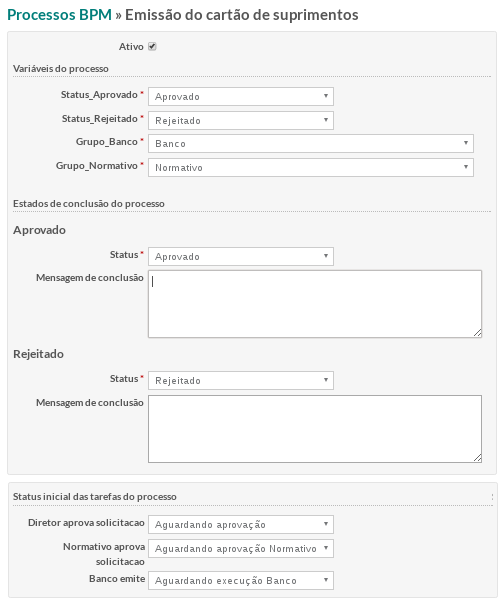
\includegraphics[width=1\textwidth]{imagens/plugin_process_settings1.png}
\caption{Tela de configurações do processo - Variáveis}
\label{fig:plugin_process_settings}
\end{figure}

\begin{figure}[H]
\centering
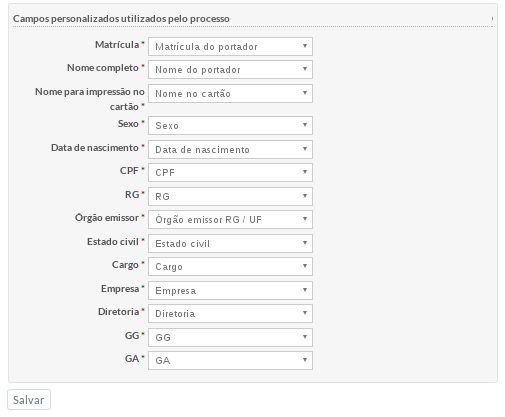
\includegraphics[width=1\textwidth]{imagens/plugin_process_settings2.png}
\caption{Tela de configurações do processo - Campos personalizados}
\label{fig:plugin_process_settings}
\end{figure}

\subsubsection{Tarefas humanas}\label{sec:integracao_redmine_activiti_implementacao_detalhes_desenvolvimento_sincronizacao_human_task}

Como dito no capítulo  \ref{chp:bpm}, as tarefas humanas do Activiti BPM são representadas no Redmine por subtarefas das tarefas que representam processos. Assumimos que todo processo do Activiti BPM configurado no Redmine possui tarefas humanas, uma vez que o principal objetivo é ajudar o usuário a interagir com o processo.
Quando uma tarefa humana é criada no decorrer do processo, o Redmine precisa refletir isto, de modo que esta tarefa possa ser executada pelo ator correto e o processo siga seu curso. O espelhamento desta tarefa no Redmine é totalmente automatizado, através de um job que roda a cada 5 minutos e verifica se existem tarefas humanas abertas que não foram espelhadas, para cada processo ativo no Redmine. Os valores dos campos do processo de uma tarefa são populados nos campos padrão e campos personalizados conforme configurados na tela exibida na figura \ref{fig:plugin_process_settings}

\section{Customização do Activiti BPM}\label{sec:integracao_redmine_activiti-implementacao-activiti}

A integração entre o Redmine e o Activiti BPM foi desenvolvida sob o aspecto de direcionar a maior parte das customizações para o lado do Redmine, uma vez que esta é apenas uma das possibilidades de interface com o motor de processos. Num cenário mais amplo de processos mais complexos, outros tipos de dispositivos ou sistemas poderiam realizar uma comunicação direta com os processos.

A API REST padrão oferecida pelo Activiti BPM foi utilizada para a integração entre as ferramentas, uma vez que é bem completa e oferece a maioria dos serviços necessários para a comunicação. Também contou a facilidade de chamadas a APIs REST pelo Ruby on Rails. 

Entretanto, identificamos a ausência de um serviço fundamental para integração entre as ferramentas. Esse serviço deveria retornar uma lista contendo as definições de tarefas contidas em um determinado processo, incluindo os campos disponíveis nos formulários das tarefas. Essa definição nos permitiria estabelecer a interface para o mapeamento dos campos do processo com os campos das tarefas do Redmine.

Sendo assim, extendemos a API REST do Activiti BPM, através da criação de um classe Java representando um novo serviço, semelhante aos serviços existentes no seu código-fonte. Esse serviço consistiu no consumo de uma API Java já disponibilizada pelo Activiti BPM, mas ausente na API REST. O código-fonte pode ser consultado no apêndice \ref{code:task_definition_service}.

\section{Resultados}\label{sec:integracao_redmine_activiti-resultados}